% Autor: Leonhard Segger, Alexander Neuwirth
% Datum: 2017-10-30
\documentclass[
	% Papierformat
	a4paper,
	% Schriftgröße (beliebige Größen mit „fontsize=Xpt“)
	12pt,
	% Schreibt die Papiergröße korrekt ins Ausgabedokument
	pagesize,
	% Sprache für z.B. Babel
	ngerman
]{scrartcl}

% Achtung: Die Reihenfolge der Pakete kann (leider) wichtig sein!
% Insbesondere sollten (so wie hier) babel, fontenc und inputenc (in dieser
% Reihenfolge) als Erstes und hyperref und cleveref (Reihenfolge auch hier
% beachten) als Letztes geladen werden!

\usepackage{tikz}
\usetikzlibrary{calc,patterns,angles,quotes} % loads some tikz extensions\usepackage{tikz}
\usetikzlibrary{babel}

% Silbentrennung etc.; Sprache wird durch Option bei \documentclass festgelegt
\usepackage{babel}
% Verwendung der Zeichentabelle T1 (Sonderzeichen etc.)
\usepackage[T1]{fontenc}
% Legt die Zeichenkodierung der Eingabedatei fest, z.B. UTF-8
\usepackage[utf8]{inputenc}
% Schriftart
\usepackage{lmodern}
% Zusätzliche Sonderzeichen
\usepackage{textcomp}

% Mathepaket (intlimits: Grenzen über/unter Integralzeichen)
\usepackage[intlimits]{amsmath}
% Ermöglicht die Nutzung von \SI{Zahl}{Einheit} u.a.
\usepackage{siunitx}
% Zum flexiblen Einbinden von Grafiken (\includegraphics)
\usepackage{graphicx}
% Abbildungen im Fließtext
\usepackage{wrapfig}
% Abbildungen nebeneinander (subfigure, subtable)
\usepackage{subcaption}
% Funktionen für Anführungszeichen
\usepackage{csquotes}
\MakeOuterQuote{"}
% Zitieren, Bibliografie
\usepackage[sorting=none]{biblatex}


% Zur Darstellung von Webadressen
\usepackage{url}
%chemische Formeln
\usepackage[version=4]{mhchem}
% siunitx: Deutsche Ausgabe, Messfehler getrennt mit ± ausgeben
\usepackage{floatrow}
\floatsetup[table]{capposition=top}
\usepackage{float}
% Verlinkt Textstellen im PDF-Dokument
\usepackage[unicode]{hyperref}
% "Schlaue" Referenzen (nach hyperref laden!)
\usepackage{cleveref}
\sisetup{
	locale=DE,
	separate-uncertainty
}
\bibliography{BA-C-04_V05_08-04-2019_References}

\begin{document}

	\begin{titlepage}
		\centering
		{\scshape\LARGE Versuchsbericht zu \par}
		\vspace{1cm}
		{\scshape\huge V05 - Lebensdauermessung eines $\gamma$-Niveaus \par}
		\vspace{2.5cm}
		{\LARGE Gruppe BA-C-04 \par}
		\vspace{0.5cm}

		{\large Alexander Neuwirth (E-Mail: a\_neuw01@wwu.de) \par}
		{\large Leonhard Segger (E-Mail: l\_segg03@uni-muenster.de) \par}
		\vfill

		durchgeführt am 08.04.2019\par
		betreut von\par
		{\large Raffaela Busse} \par %TODO Ich würde die hier legit rausnehmen. Die hat halt offiziell nur zugeschaut (und auch faktisch)
		und \par
		{\large Daniel Guderian}
		\vfill

		{\large \today\par}
	\end{titlepage}
	\tableofcontents
	\newpage

	%TODO mehr TODO in Default

	\section{Kurzfassung}
	% Hypothese	und deren Ergebnis, wenn Hypothese ist, dass nur Theorie erfüllt, sagen: Erwartung: Theorie aus einführung (mit reflink) erfüllt
	% Ergebnisse, auch Zahlen, mindestens wenn's halbwegs Sinn ergibt
	% Was wurde gemacht
	% manche leute wollen Passiv oder "man", manche nicht

  \section{Theorie}
	% wdh. Texte
	% wdh. Besprechung
	\subsection{Zerfall von Titan-44}

	Das Zerfallsschema von Titan-44 ist in \cref{fig_Zerfallsschema} dargestellt. Titan-44 zerfällt über Elektroneneinfang mit einer Halbwertszeit von \SI{2,44}{} Tagen zu einem angeregten Niveau von Scandium-44. \cite{Anleitung} %TODO ist das Halbwertszeit oder mittlere Lebensdauer???
	Das angeregte Scandium-44 sendet dann zwei $\gamma$-Photonen beim Abregen auf das zu untersuchende mittlere Niveau und dann in den Grundzustand aus.
	%Hierbei ist zu erwähnen, dass die erste Abregung mit einer Halbwertszeit von \SI{0,15}{\mikro \seconds} stattfindet %nvm schätze das ist doch egal. %TODO oder muss man hier wissen, dass das nicht lange in dem oberen Niveau ist, wir hatten irgendwas bei der Vorbesprechung gesagt, aber war glaube ich halbgar
	Der Grundzustand von Scandium-44 zerfällt dann durch Beta-Plus-Zerfall in einen angeregten Zustand von Calcium-44, der dann wiederum durch Aussenden eines $\gamma$-Photons in den Grundzustand über.
	Für die Versuchsdurchführung sind die beiden Photonen bei der Abregubg des Scandiums und der Beta-Plus-Zerfall relevant.

	\begin{figure}[H]
			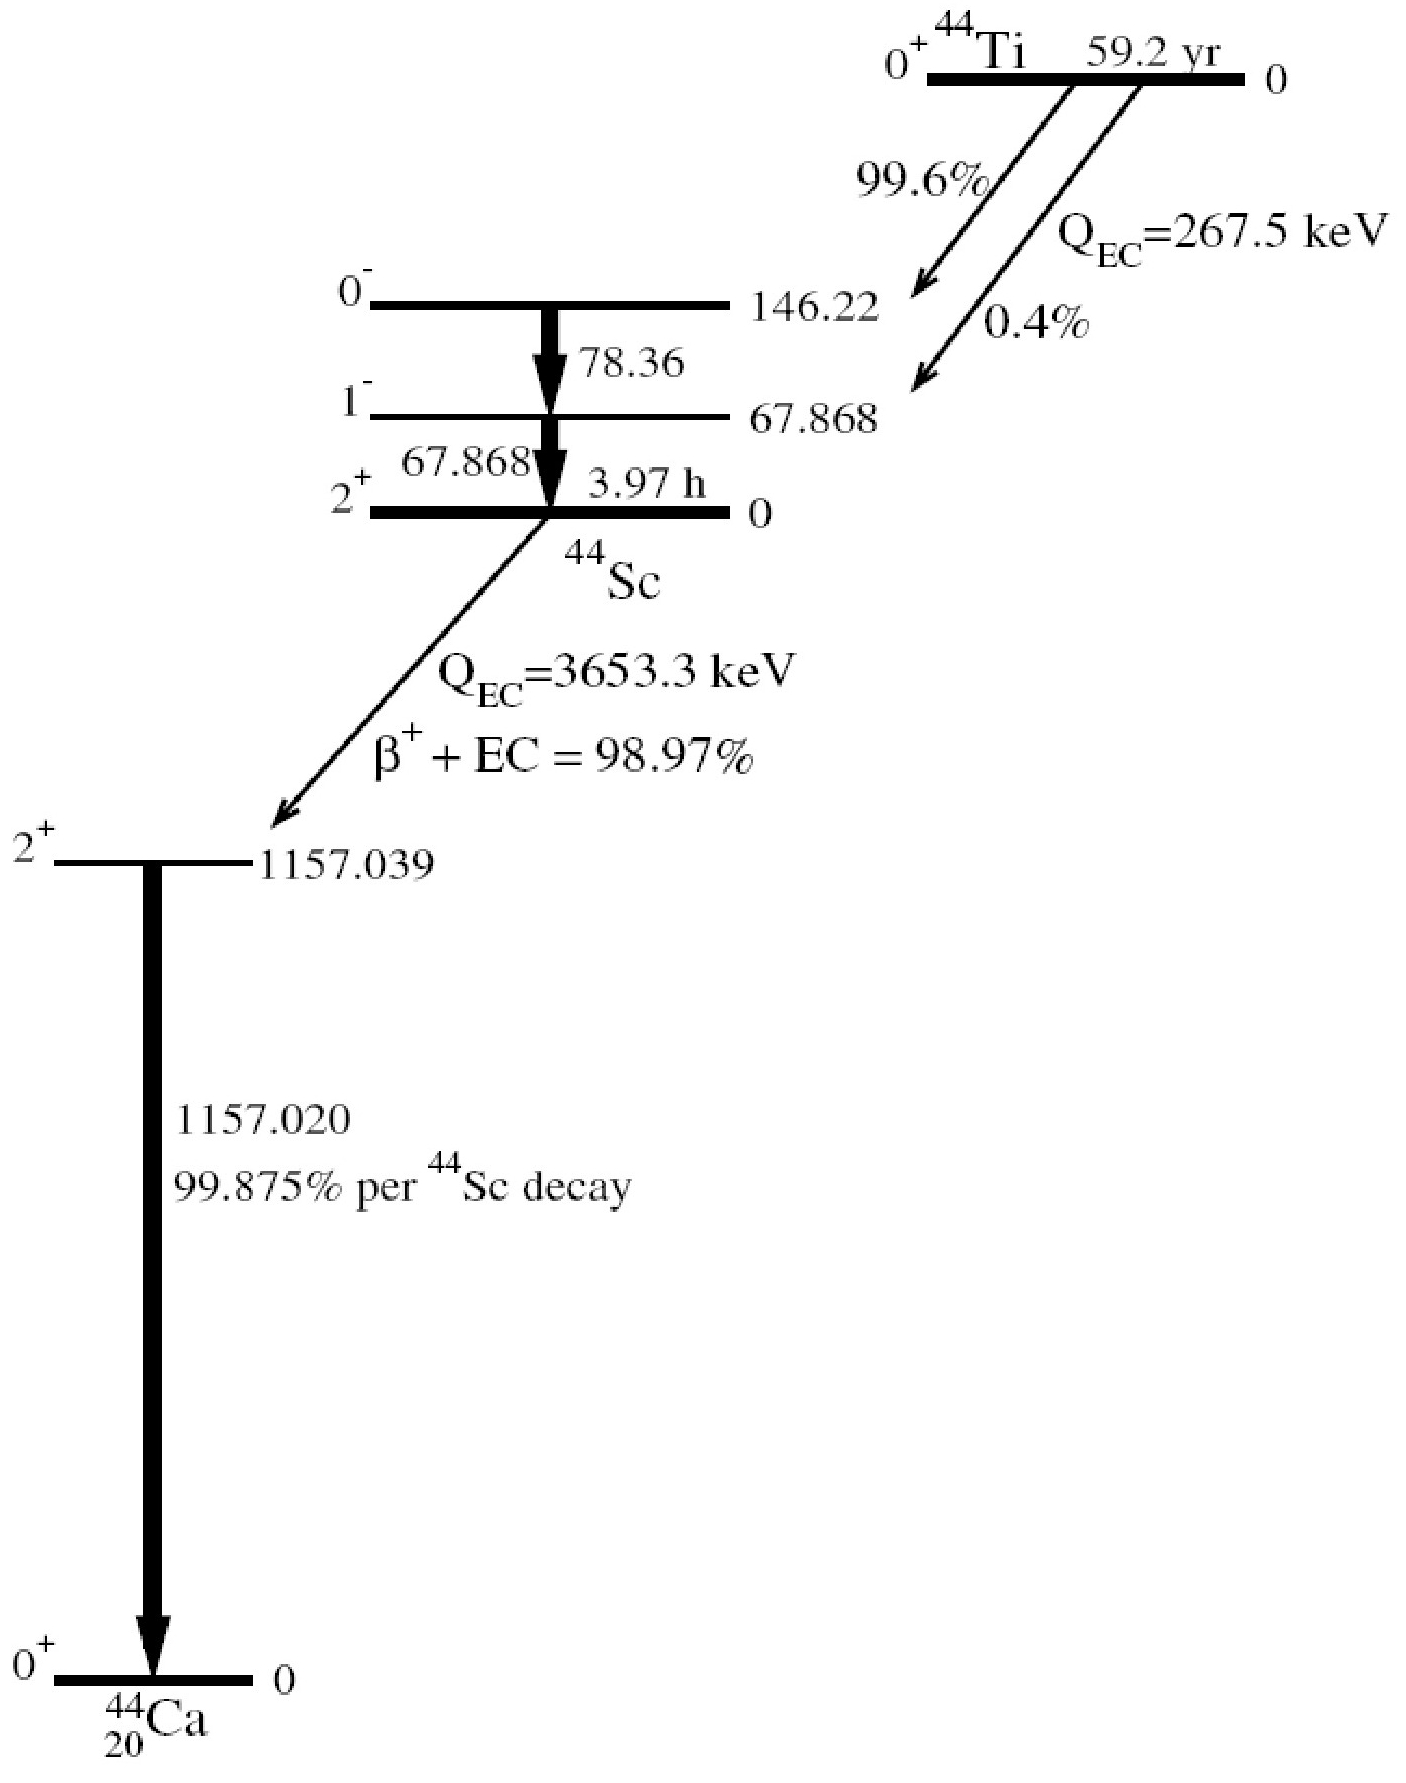
\includegraphics[width=0.6\linewidth]{img/44Ti-decay_reduziert}
			\caption{
			Reduziertes Zerfallsschema von Titan-44 über Scandium-44 zu Calcium-44. Zerfallswege geringer Wahrscheinlichkeit sind nicht dargestellt.
			\cite{Zerfallsschema} %TODO theoretisch copyrightmäßig schwierig, weil ich den unnötigen Teil rausgecropt habe. Alternative: Anleitung scannen.
			}
			\label{fig_Zerfallsschema}
	\end{figure}

	\subsection{Elektroneneinfang}
	%TODO Elektroneneinfang erklären bzw Gleichung hinschreiben!
	\subsubsection{Beta-Plus-Zerfall}
	Wie oben beschrieben findet die folgende Kernreaktion statt:
	\begin{equation}
		\label{eq_beta-plus}
		 _{21}^{44}\text{Sc} \rightarrow _{20}^{44}\text{Ca} + \text{e}^+ + \nu_{\text{e}}
	\end{equation}
	Das dabei entstandene Positron wird durch Wechselwirkung mit dem Rest der Probe abgebremst.
	Wenn es ausreichend stark abgebremst ist, kann es mit einem Elektron in der Probe das instabile Positronium bilden.
	Beim Positronium unterscheidet man je nach Spinausrichtung von Positron und Elektron in Parapositronium ($S=0$) und Orthopositronium ($S=1$).
	Aufgrund von Spin- und Impulserhaltung zerfällt Orthopositronium in eine ungerade Anzahl Photonen, die mindestens \num{3} beträgt.
	Aus analogen Gründen zerfällt Parapositronium eine gerade Anzahl Photonen, aber mindestens \num{2}.
	Da Zerfälle, die die Produktion einer geringeren Menge an Photonen vorraussetzt, wahrscheinlicher sind, zerfällt Orthopositronium deutlich langsamer als Parapositronium.
	Gleichzeitig kann durch Umgebungswechselwirkung Orthopositronium in Parapositronium übergehen, was während der vergleichsweise langen Zerfallsdauer wahrscheinlich ist.
	Deswegen kann man sich in den folgenden Betrachtungen im Wesentlichen auf den Zerfall von Parapositronium in zwei Photonen mit einer Energie von \SI{511}{keV} beschränken.
	Außerdem ist anzumerken, dass die mittlere Lebensdauer von Parapositronium bei \SI{125}{ps} liegt, was im Vergleich zur erwarteten Lebensdauer des untersuchten $\gamma$-Niveaus verschwindend gering ist. \cite{Anleitung}

	%TODO Wechselwirkungen
	\section{Methoden}
	% Bilder von der Website klauen
	% einer will Präsens
	%TODO Detektionsmechanismus
	%TODO welche Geräte haben welche Funktion

	%TODO  Zeiten
	% Zeitdifferenz: 25.3h
	% Positronium_Zeitdifferenz: 1.2h
	% Zeitkalibrierung: 7s
	% Energy_Start: 3.7m
	% Energy_Stop: 11.4m

	%TODO
	% Zeit in Material bei Speed of Light vernachläsigbar (bzw. Ausdehnung)

	\section{Ergebnisse und Diskussion}
	%TODO Unsicherheiten


	\subsection{Beobachtung und Datenanalyse}
	% Allgemeine Beobachtungen
	% Einflüsse von veränderten Parametern auf Messung
	\subsubsection{Unsicherheiten}
	% Berechung nach Aufgabenstellung

	\subsection{Energiespektren}
	Zuächst wurden die Energeispektren \cref{fig_energy_start} und \cref{fig_energy_stop} gemessen. Hieraus wurden die Kanalbereiche für aus dem jeweiligen Prozess stammende Photonen ermittelt.

	%TODO Peaks der zwei Zerfälle nicht unterscheidbar

	\begin{figure}[H]
				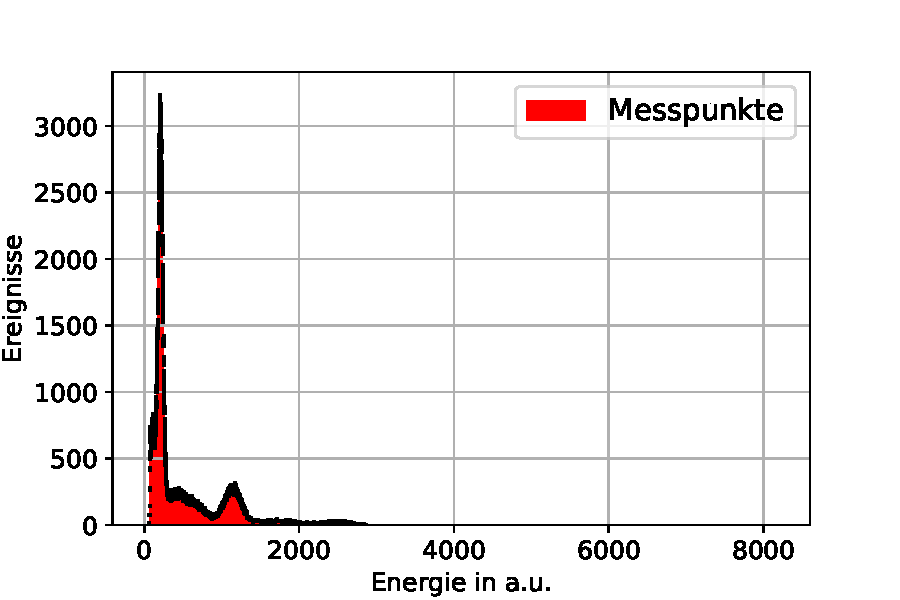
\includegraphics[width= 0.9 \linewidth]{img/Energiespektrum_Start}
				\caption{
				Energiespektrum welches von der ersten Messapparatur aufgenommen wurde.
				Die Unsicherheiten sind in Schwarz abgebildet, sodass sich der Messwert mittig im schwarzen Bereich befindet.
				}
				\label{fig_energy_start}
		\end{figure}

	\begin{figure}[H]
				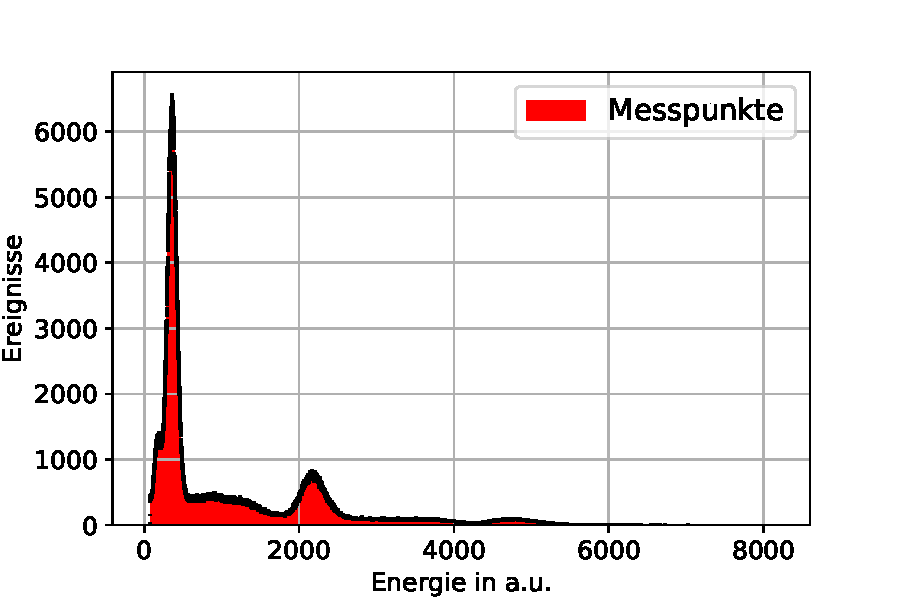
\includegraphics[width= 0.9 \linewidth]{img/Energiespektrum_Stop}
				\caption{
				Energiespektrum welches von der zweiten Messapparatur aufgenommen wurde.
				Die Unsicherheiten sind in Schwarz abgebildet, sodass sich der Messwert mittig im schwarzen Bereich befindet.
				}
				\label{fig_energy_stop}
		\end{figure}

  \subsubsection{Zeitkalibrierung}
	Der Mittelwert der Abstände der Peaks in \cref{fig_zeitkalibrierung} beträgt \SI{514.8+-0.4}{}, das heißt so viele Kanäle entsprechen einer Zeit von \SI{0.64+-0.003}{\mu s}.

	\begin{figure}[H]
				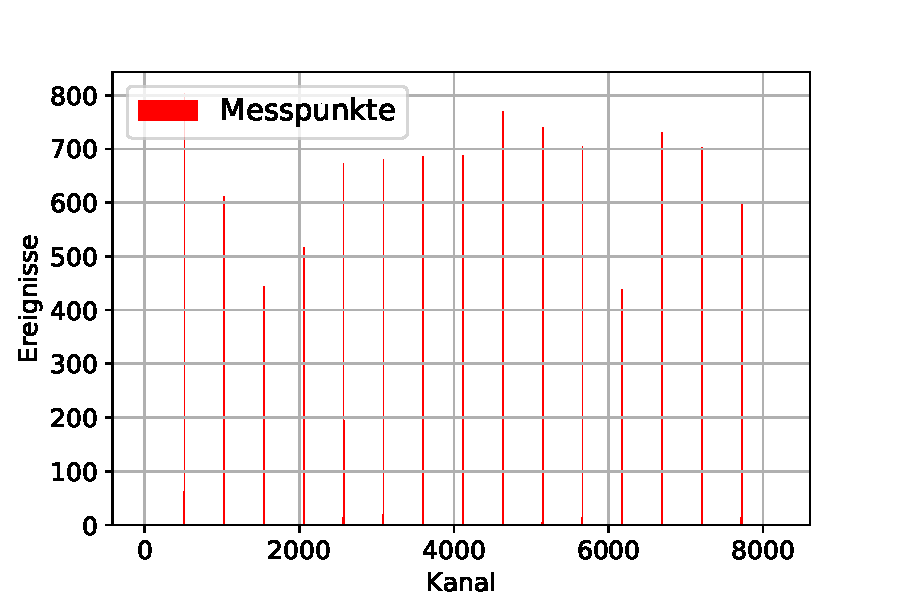
\includegraphics[width= 0.9 \linewidth]{img/Zeitkalibrierung}
				\caption{
				Zeitkalibrierung der Kanäle mittels eines Zeitkalibrators %TODO 'TIME Calibrator' ?
				Es gibt auch kleine Beiträge zu anderen Kanälen in naher Umgebung der Peaks, jedoch sind diese wegen der Auflösung des Bildes kaum sichtbar.
				}
				\label{fig_zeitkalibrierung}
		\end{figure}

		\subsubsection{Bestimmung des Nullpunkts}
		In \cref{fig_positronium_zeitdifferenzen} sind die Messungen der Zeitdifferenzen des Positroniumzerfalls abgebildet.
		Da dieser sehr scharf ist, ist er in \cref{fig_positronium_zeitdifferenzen_zoom} vergrößert dargestellt.
		Es wird eine Gaußfunktion \ref{eq_gauss} an die Messpunkte angepasst.
		\begin{equation}
			\label{eq_gauss}
			%A * np.exp(-(x - x0)**2 / 2 / d**2)
			 f(t) = N\exp\left\{{\frac{(t-T_0)^2}{2 \Delta T^2}}\right\}
		\end{equation}
		Die Standardabweichung des Fits $\Delta T$ beschreibt für die folgende Bestimmung der Lebensdauer des $\gamma$-Niveaus die Unsicherheit der Messapparatur bei der Auflösung von Zeitdifferenzen, da beim Positroniumzerfall kein zeitlicher Unterschied vorliegt. %TODO ref in Theorie? bzw. vernachlässigbar klein

	\begin{figure}[H]
				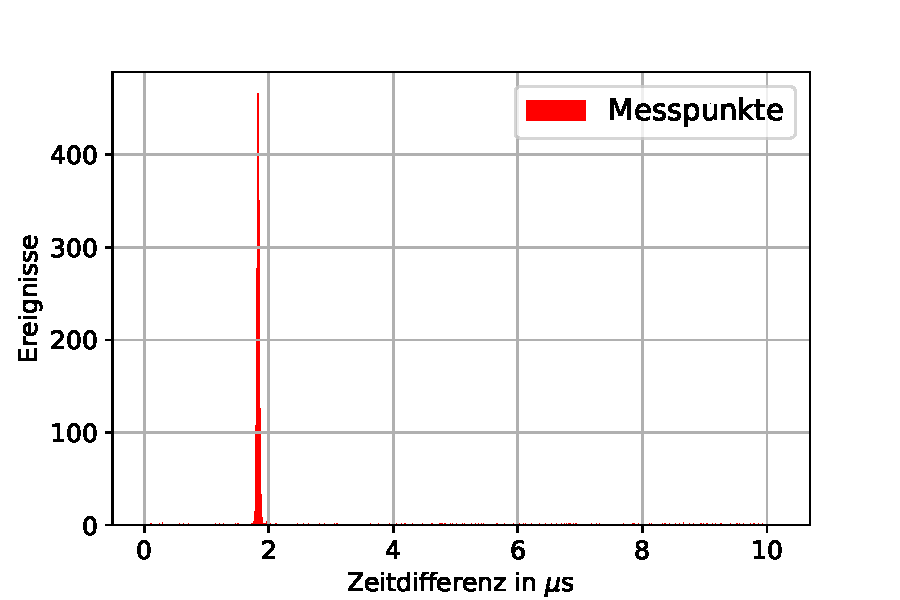
\includegraphics[width= 0.9 \linewidth]{img/Positronium_Zeitdifferenz}
				\caption{
					Positronium-Kanal
				Die Unsicherheiten sind in Schwarz abgebildet, sodass sich der Messwert mittig im schwarzen Bereich befindet.
				}
				\label{fig_positronium_zeitdifferenzen}
		\end{figure}

	\begin{figure}[H]
				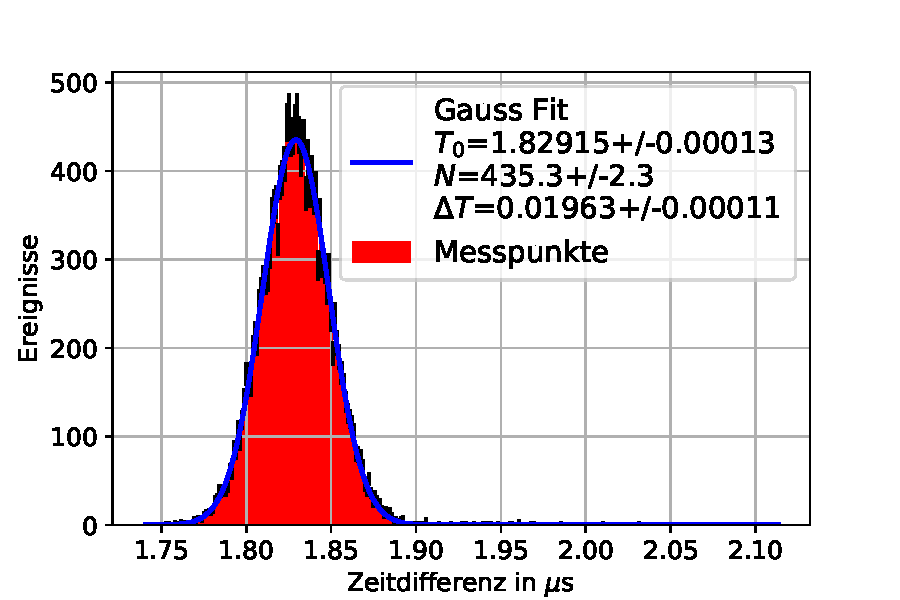
\includegraphics[width= 0.9 \linewidth]{img/Positronium_Zeitdifferenz_zoom}
				\caption{
					Positronium-Kanal:
				Die Unsicherheiten sind in Schwarz abgebildet, sodass sich der Messwert mittig im schwarzen Bereich befindet.
				}
				\label{fig_positronium_zeitdifferenzen_zoom}
		\end{figure}

		\subsubsection{Bestimmung der Lebensdauer}

		\subsubsection*{Abschätzung}
		Mit \cref{fig_zeitdifferenz_zoom} wurde die Halbwertszeit grob abgeschätzt.
		Hierbei beschreibt die grüne Horizontale bei \SI{125}{} Ereignissen den Untergrund (siehe \cref{fig_zeitdifferenz}).
		In gelb verlaufen eine Horizontale und eine Vertikale durch das abgeschätze Maximum.
		Ebenso ist der Punkt der mit halb so vielen Ereignissen (ohne den Untergrund) lila markiert.
		Die Differenz gibt die Halbwertszeit $t_{1/2}=\SI{150+-50}{ns}$.
		\begin{figure}[H]
				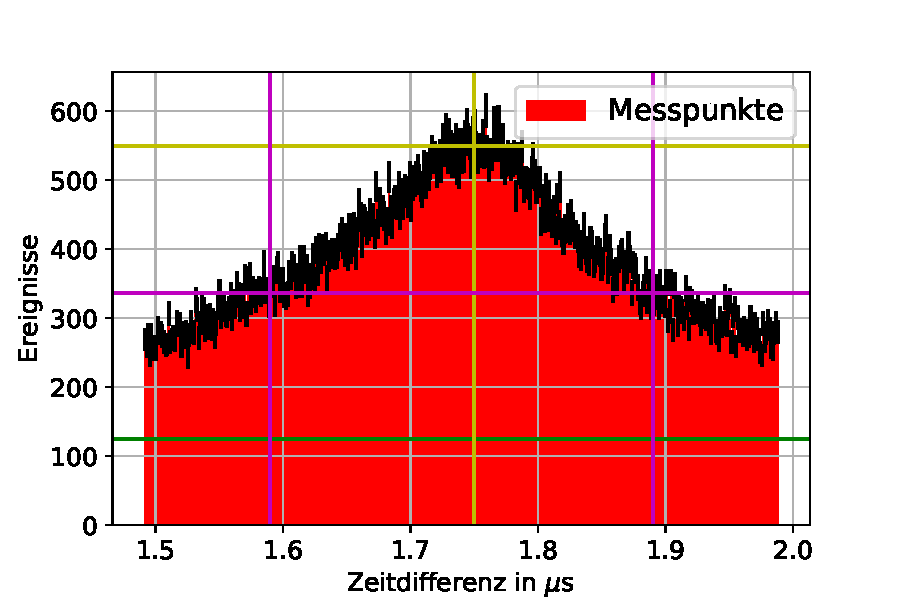
\includegraphics[width= 0.9 \linewidth]{img/Zeitdifferenzen_zoom}
				\caption{
					$\gamma$-Niveau-Kanal:
				Die Unsicherheiten sind in Schwarz abgebildet, sodass sich der Messwert mittig im schwarzen Bereich befindet.
				}
				\label{fig_zeitdifferenz_zoom}
		\end{figure}
		\subsubsection*{Fit}
		In \cref{fig_zeitdifferenz} ist die Grüne Linie der Mittelwert aller Ereignisse bei einer Zeitdifferenz größer \SI{4}{\mu s}.
		Der lila Fit ist in in die jeweilige Richtung ein exponentiell abfallende Funktion:
		\begin{equation}
			\label{eq_dexp}
			f(t)=N\cdot (\exp{-\left\{\lambda_1(t-T_0)\right\}}\Theta(t-T_0)+\exp{\left\{\lambda_2(t-T_0)\right\}}\Theta(T_0-t))
		\end{equation}
	\begin{figure}[H]
				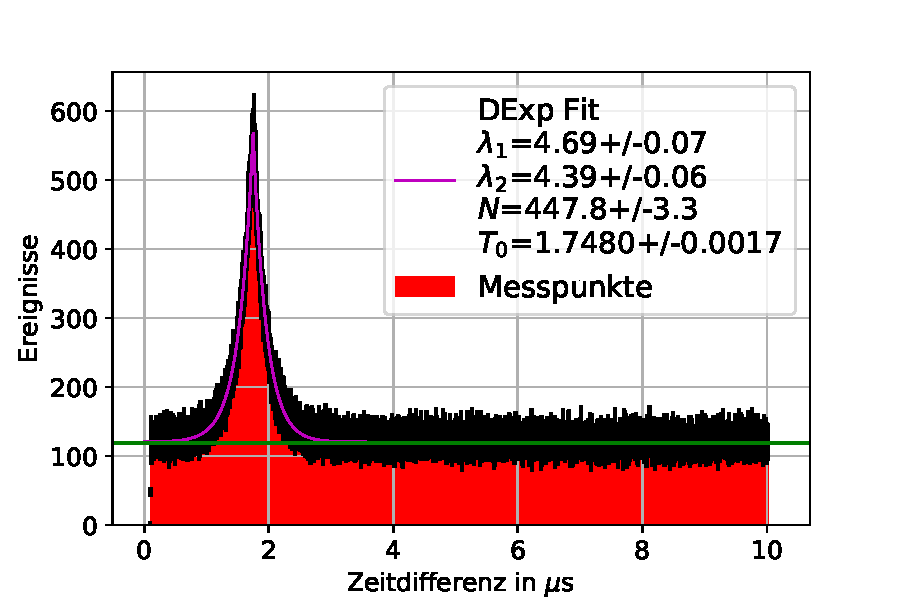
\includegraphics[width= 0.9 \linewidth]{img/Zeitdifferenzen}
				\caption{
					$\gamma$-Niveau-Kanal:
				Die Unsicherheiten sind in Schwarz abgebildet, sodass sich der Messwert mittig im schwarzen Bereich befindet.
				}
				\label{fig_zeitdifferenz}
		\end{figure}
		\subsubsection*{Integration}

		In \cref{tb_leb} sind die insgesamt resultierenden Lebensdauern aufgeführt.
		\begin{table}[H]
		\centering
		\begin{tabular}{c | c | c | c  }
			 Index&$\lambda$ in \si{\mu s^{-1}}& $\tau=1/\lambda$ in \si{ns} &$t_{1/2}=\tau\ln 2$ in \si{ns}\\ \hline
			 1&\SI{4.68+-0.07}{}&\SI{213+-3}{}&\SI{147+-2}{} \\
			 2&\SI{4.39+-0.06}{}&\SI{228+-3}{}&\SI{158+-2}{} \\
			 3\\
			 4\\
		\end{tabular}
		\caption{
		Verschiedene gemessene Lebensdauern, bzw. Halbwertszeiten, des angeregten $\gamma$-Niveaus von $^{44}$Sc.
		}
			 \label{tb_leb}
	\end{table}
	\subsection{Diskussion}
	% Bezug/Nutzen oder sonst was
	% auch hier die Hypothese wiederholen
	% keine Messwerte hier, nach manchen Menschen, zumindest "direkt" erstellte Diagramme net hier, auch wenn Lesbarkeit-bla

	\section{Schlussfolgerung}
	% Rückgriff auf Hypothese und drittes Nennen dieser

	% Quellen zitieren, Websiten mit Zugriffsdatum
	% Verweise auf das Laborbuch (sind erlaubt)
	% Tabelle + Bilder mit Beschriftung
	\printbibliography
\end{document}
